\subsection{Execution and results}
%erkl�ren, !was! wir machen, !warum! wir das machen und mit welchem ziel
%(wichtig) pr�zize erkl�ren, wie bei dem versuch vorgegangen und was gemacht wurde
In this section the execution and the results will be presented.

\subsection{Identification of the lines and measurement of the absorption}

In this measurement all 39 theoretical expected lines in the spectrum should be measured. At first the pressure for this measurement has to be around 10$^{-1}$mbar and constant. The pressure during the measurement was at 9,8$ \cdot$ 10$^{-2}$. The measurement started at the 28GHz, because the peaks in that range are bigger then the ones at the beginning of the spectrum. For the measurement of the peaks the wave meter was used. The dip from the wave meter was position right on the dip of the NH3 and the frequence was the take from the wave meter. Then the oscilloscope was used to determine the hight of the peaks. For that the dip of the wave meter was scrolled out of the visible spectrum on the oscilloscope. Then the to bars on the oscilloscope were used to determine the size of the dip. 

With the size of the dip the absolute absorption coefficient can be calculated. The absolute absorption coefficient is calculated by formula \ref{equ:alpha}. U$_0$ was not know so the coefficients where normed to the size of the the 6 6 peak, so $\alpha_{rel_{6,6}}$ = 1. All measured Date can be find in table ??.

\begin{align}
\label{equ:alpha}
\alpha_{rel} = \frac{10}{l} \cdot ln(1- \frac{U_a}{U_0})
\end{align}

\begin{table}[H]
\begin{tabular}{c|c}
l & lenght of the wave guide, 5m in this buildup \\ 
U$_a$ & the intensity without any absorption \\ 
U$_0$ & the intensity of the measured peak \\ 
\end{tabular} 
\end{table}

\begin{figure}[H]
\centering
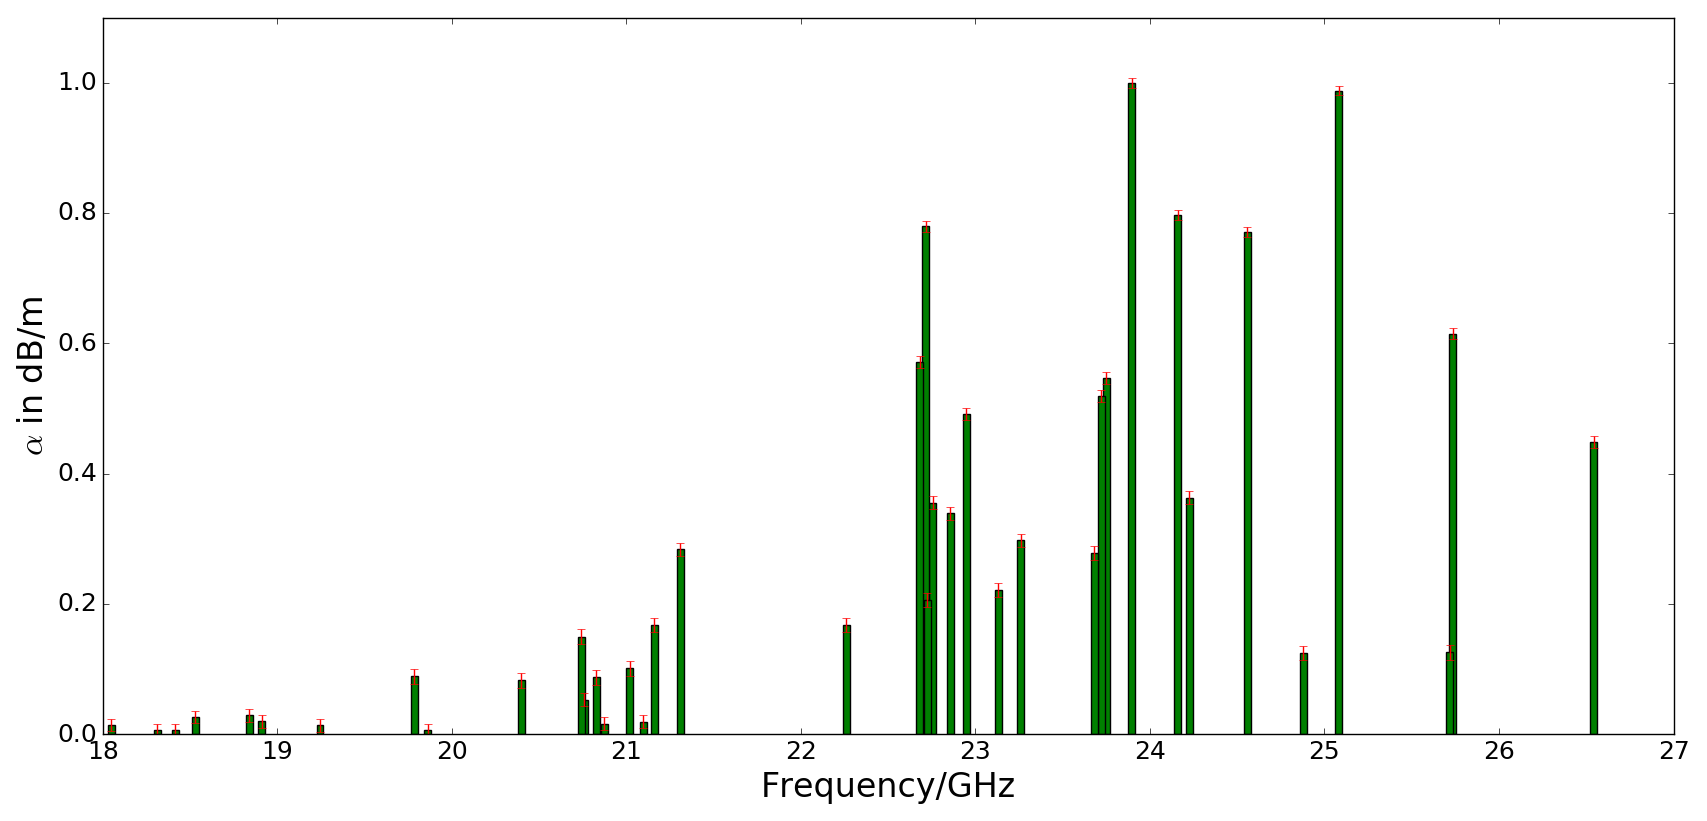
\includegraphics[scale = 0.39]{alpha.png}
\caption{The plot shows the relative absorption coefficient, the coefficient was calculated with formula ??. The errors where taken from the uncertainty of the listing}
\label{fig:alpha}
\end{figure}